\documentclass{beamer}

\title{Statistical Analysis of SST-Pyramidal Post-synaptic Amplitude Distributions}
\author{Taisuke Yasuda}

\usepackage{graphicx}

\AtBeginSubsection[]
{
  \begin{frame}<beamer>{Outline}
    \tableofcontents[currentsection, currentsubsection]
  \end{frame}
}

\DeclareMathOperator{\Bernoulli}{Bernoulli}
\DeclareMathOperator{\Lognormal}{Lognormal}

\begin{document}

\begin{frame}
  \titlepage
\end{frame}

\begin{frame}{Outline}
  \tableofcontents
  % Plan this out into sections and subsections
\end{frame}

%%%%%%%%%%%%%%%%%%%%%%%%%%%%%%%%%%%%%%%%%%%%%%%%%%%%%%%%%%%%%%%%%%%%%%%%%%%%%%%%
% Problem Set Up
%%%%%%%%%%%%%%%%%%%%%%%%%%%%%%%%%%%%%%%%%%%%%%%%%%%%%%%%%%%%%%%%%%%%%%%%%%%%%%%%

\section{Background}

\subsection{Biological Context}

\begin{frame}{Biology of Post-synaptic Amplitudes}
  % Draw a picture of how post-synaptic amplitudes work
  \begin{figure}
    \centering
    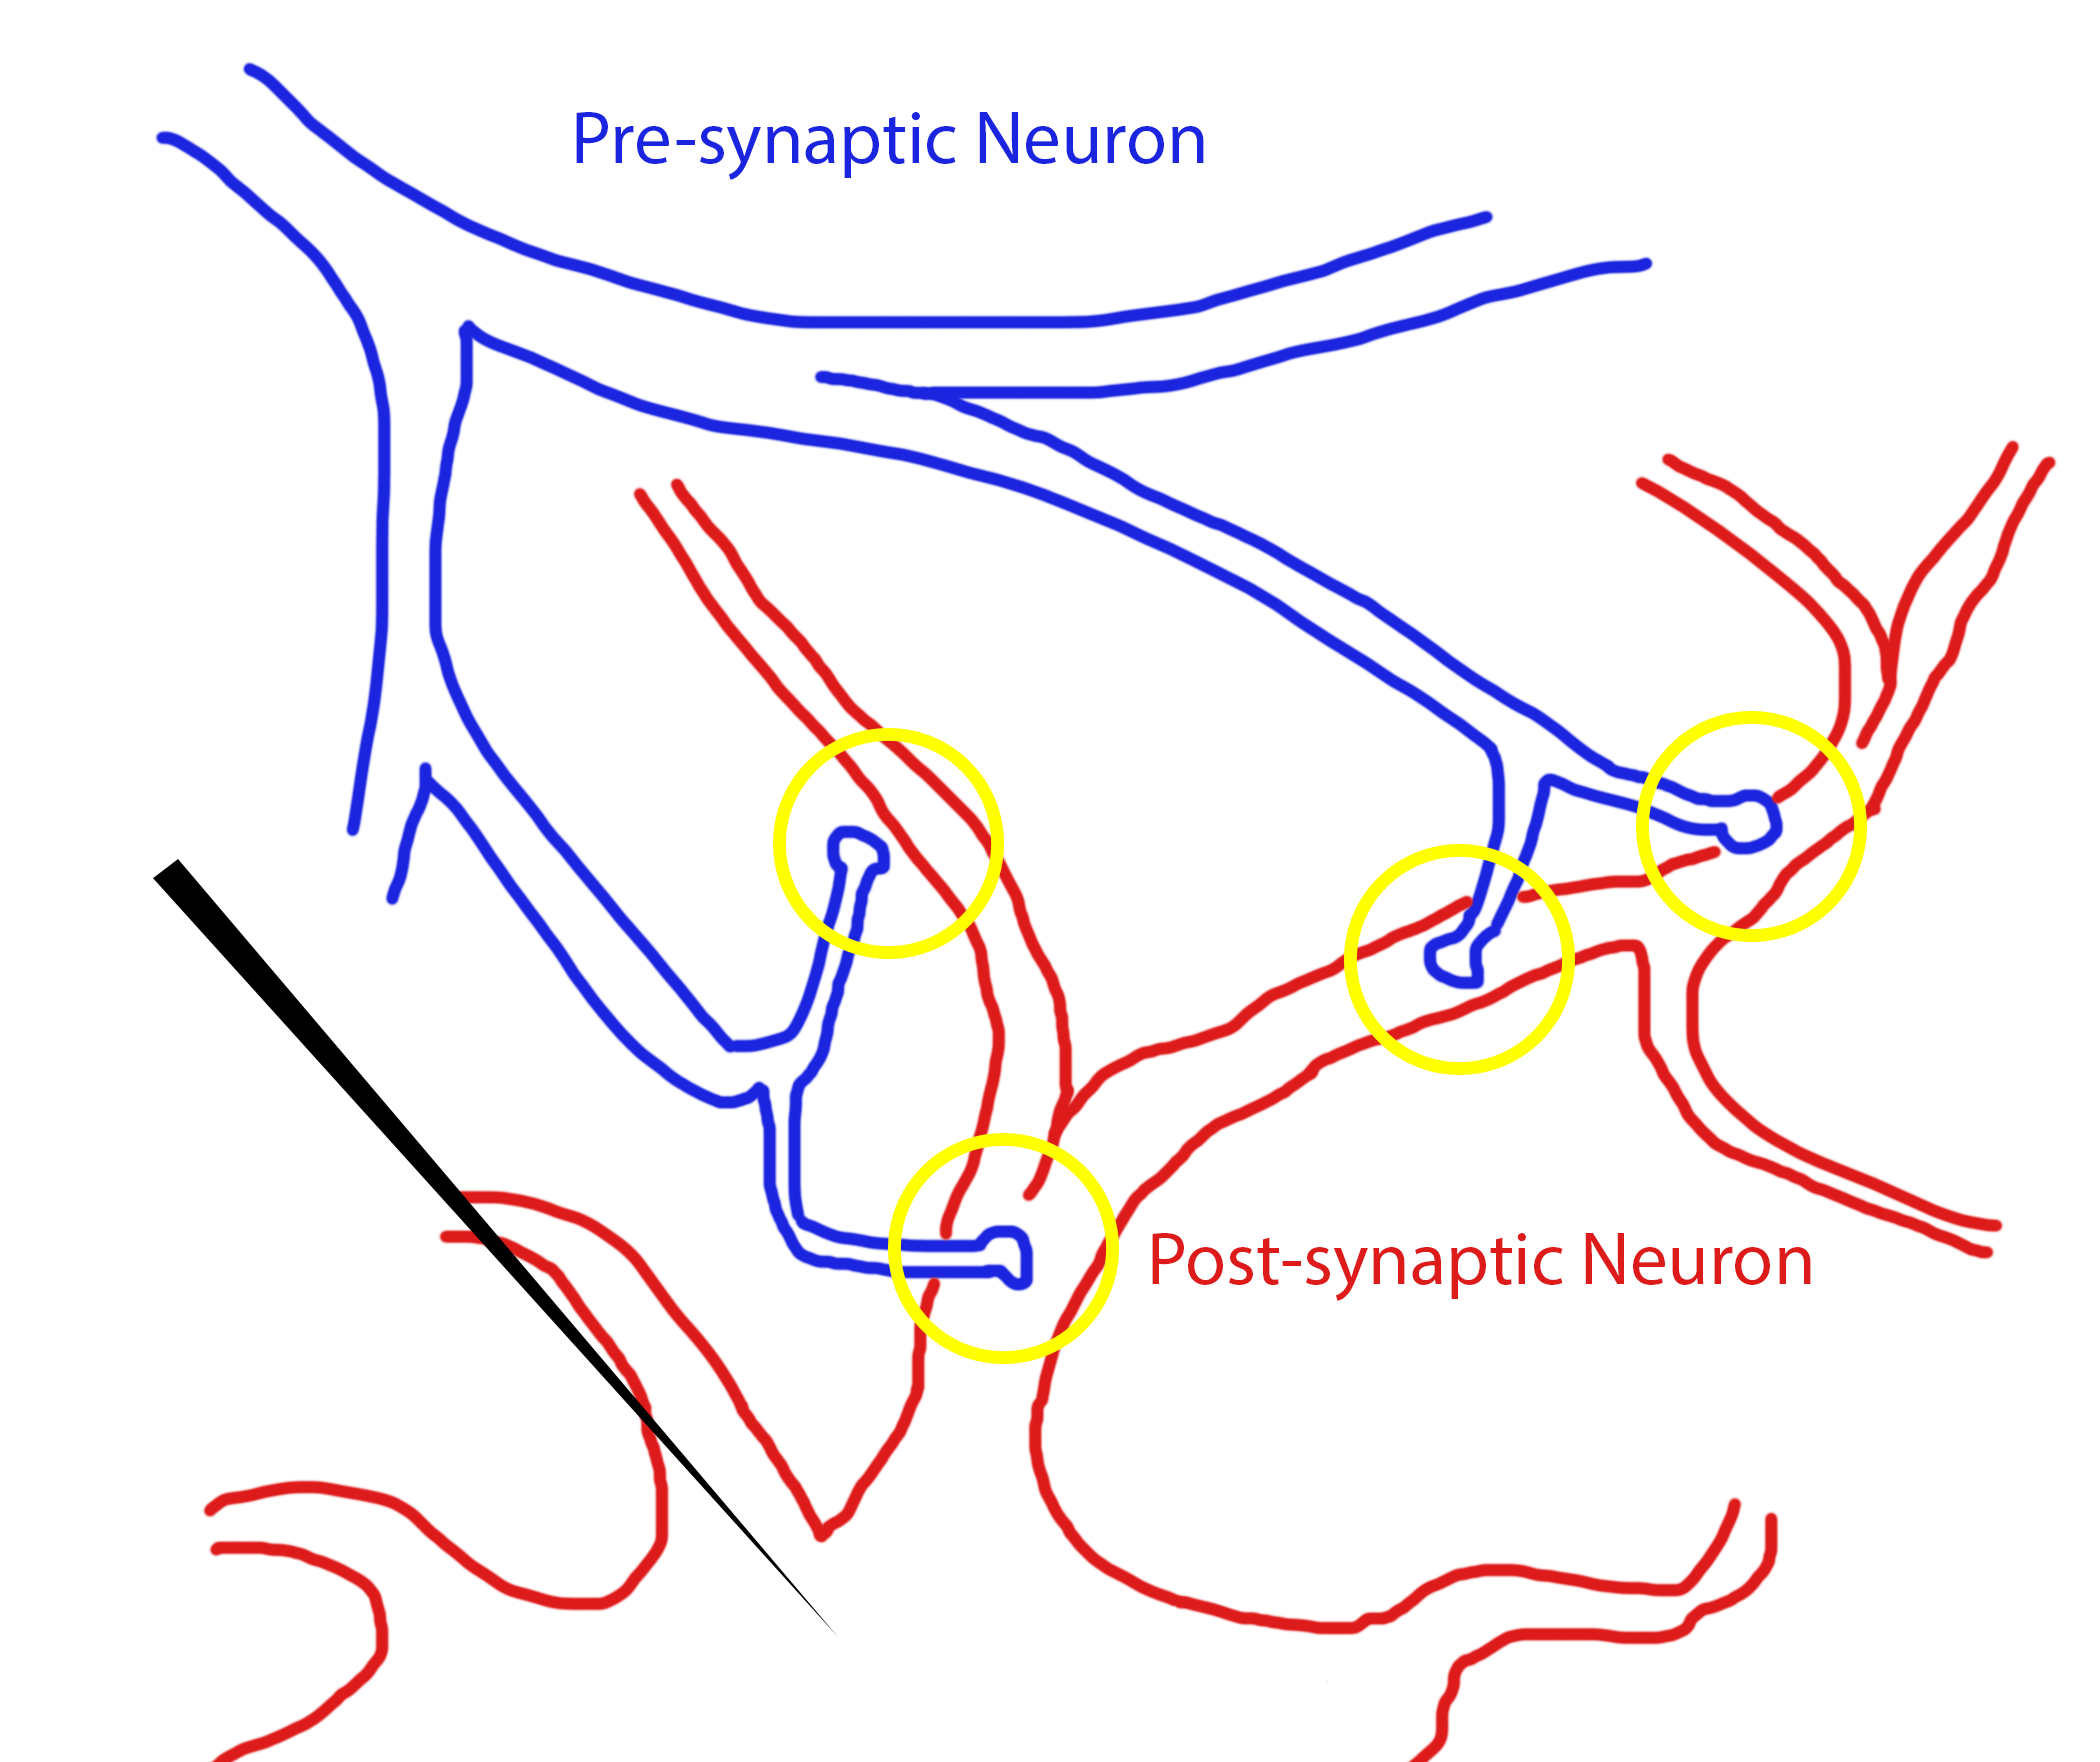
\includegraphics[width = 0.7\textwidth]{./synapse-biology.png}
    \caption{Biology of post-synaptic amplitudes}
  \end{figure}
\end{frame}

\subsection{Data Collection}

\begin{frame}{Experimental Measurements}
  % Show what we measure
  \begin{figure}
    \centering
    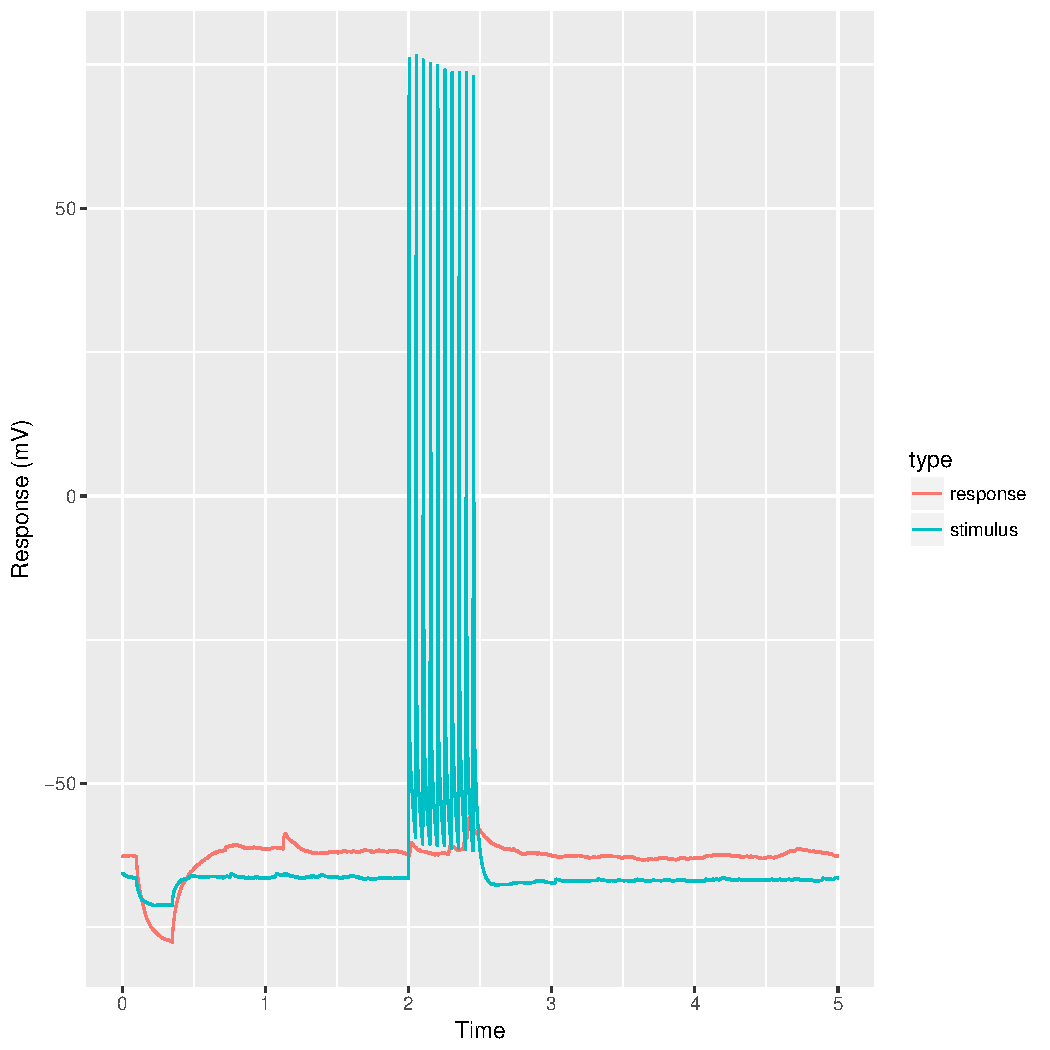
\includegraphics[width = 0.7\textwidth]{./wave-data.pdf}
    \caption{Wave files of the stimulus and response}
  \end{figure}
\end{frame}

\begin{frame}{Extracting Post-synaptic Response Amplitudes}
  % Show how to find the actual data, i.e. zoom in and find height
  \begin{figure}
    \centering
    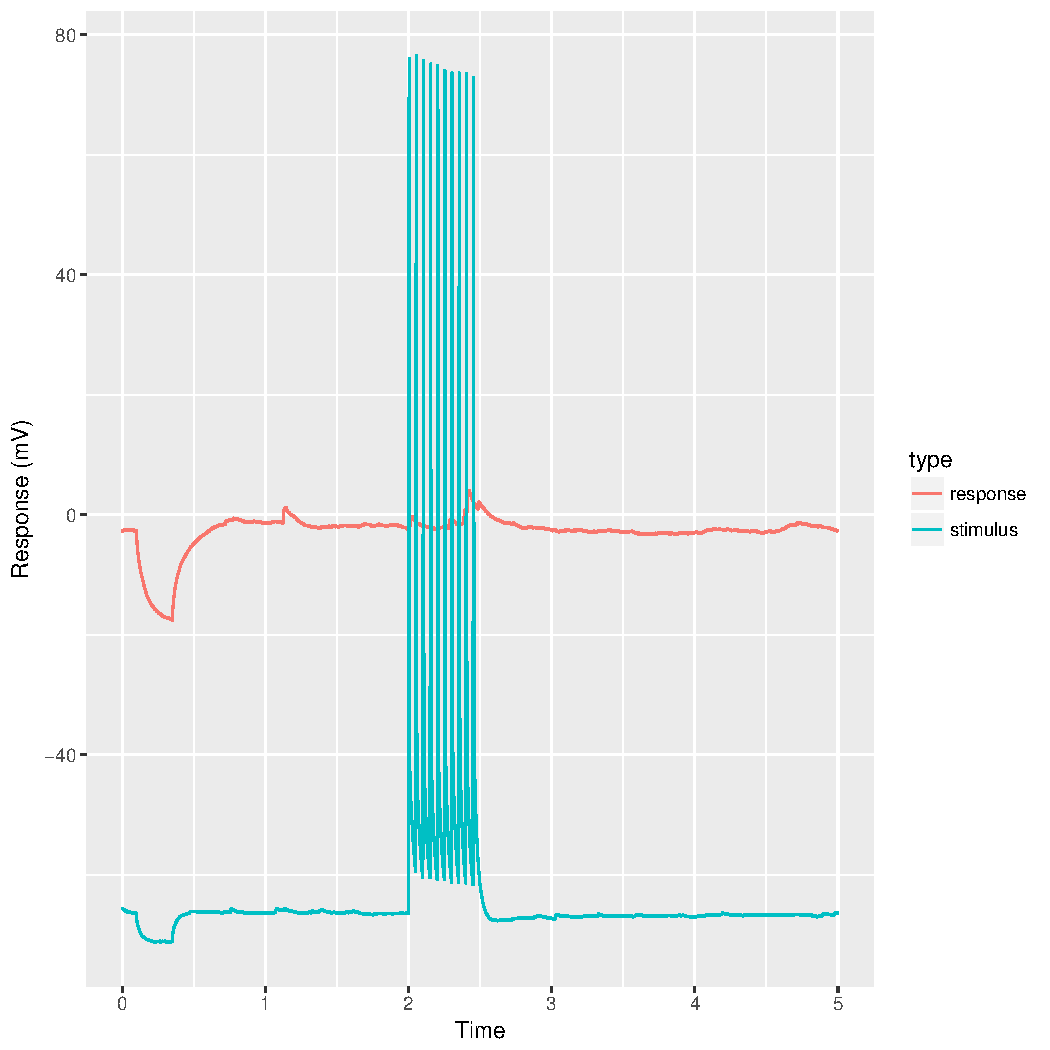
\includegraphics[width = 0.7\textwidth]{./wave-data-move.pdf}
    \caption{Moving the responses next to the stimuli}
  \end{figure}
\end{frame}

\begin{frame}{Extracting Post-synaptic Response Amplitudes}
  % Show how to find the actual data, i.e. zoom in and find height
  \begin{figure}
    \centering
    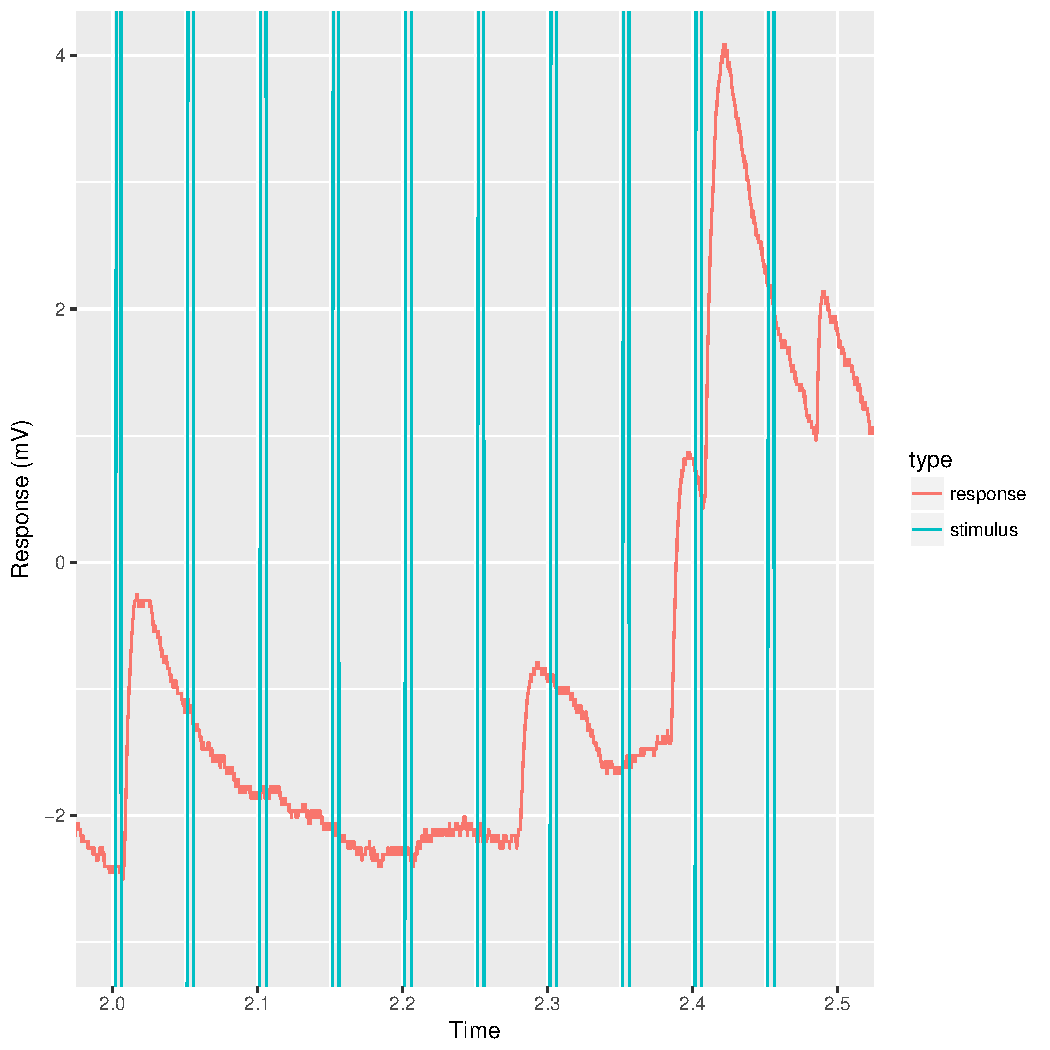
\includegraphics[width = 0.7\textwidth]{./wave-data-zoom.pdf}
    \caption{Zooming in on the stimuli and responses}
  \end{figure}
\end{frame}

\begin{frame}{Extracting Post-synaptic Response Amplitudes}
  % Show how to find the actual data, i.e. zoom in and find height
  \begin{figure}
    \centering
    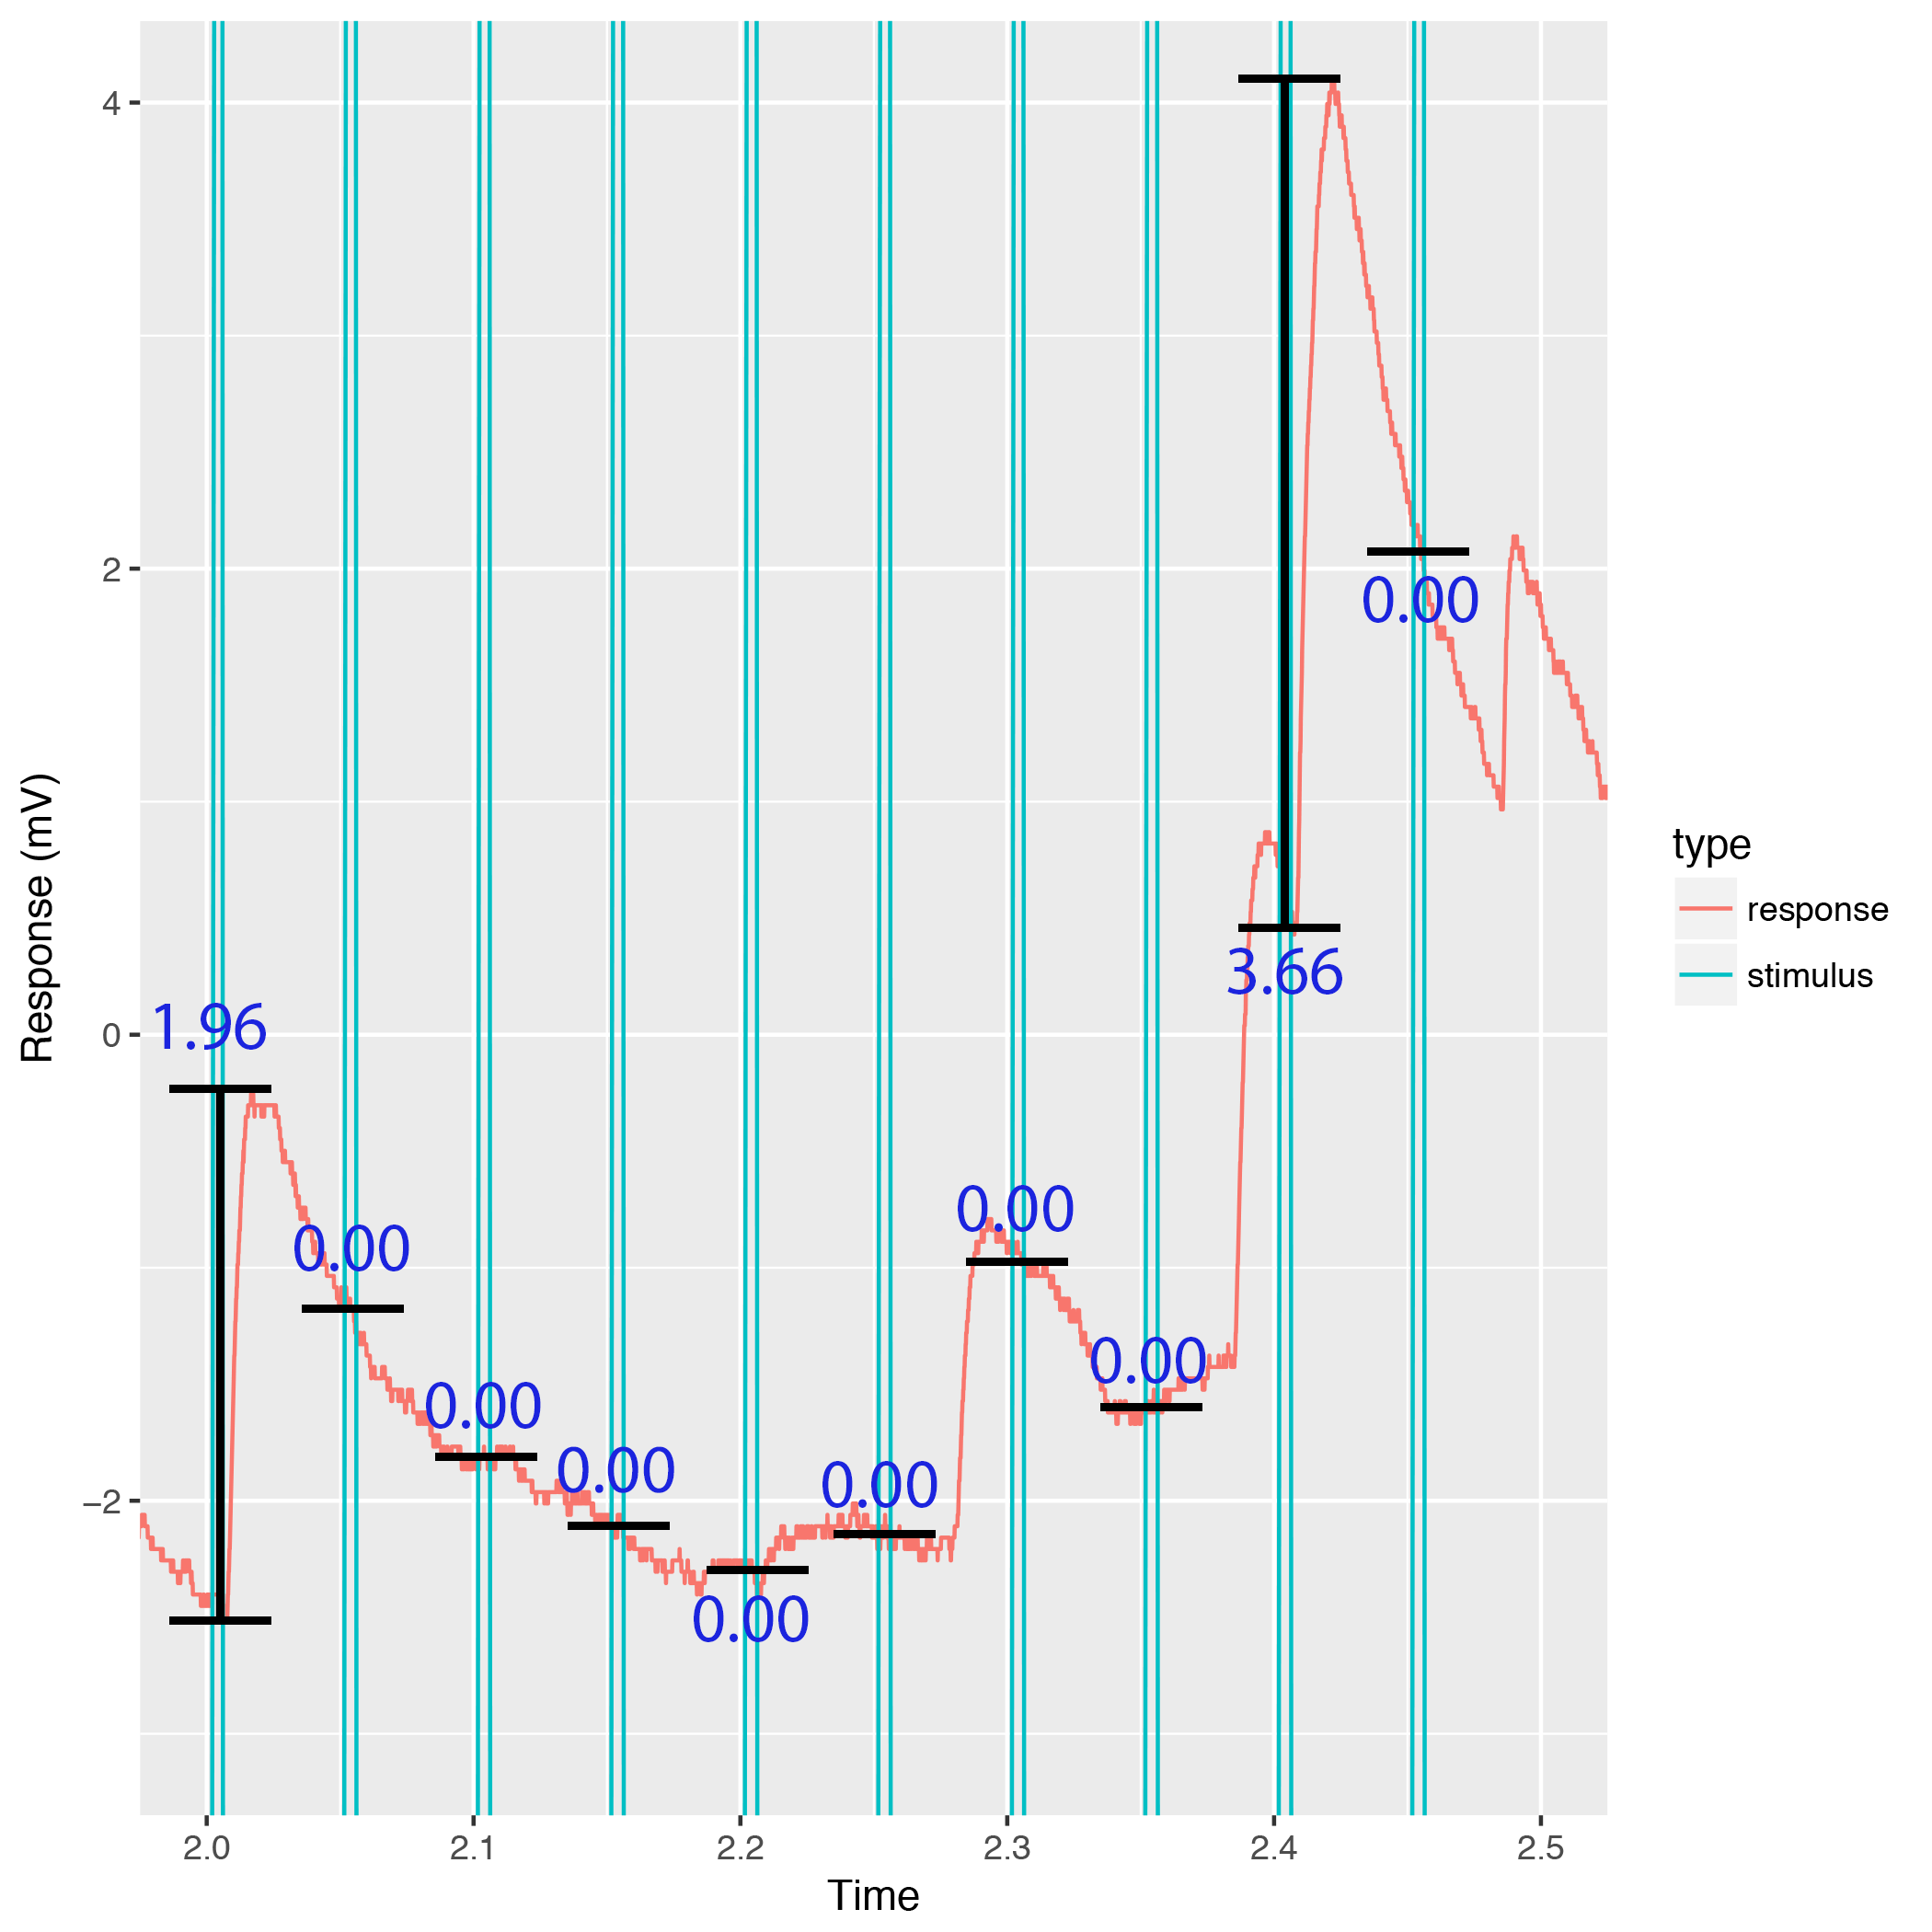
\includegraphics[width = 0.7\textwidth]{./label-wave-data.png}
    \caption{Extracting the response amplitudes}
  \end{figure}
\end{frame}

\begin{frame}{A More Typical Wave Response}
  % Cell with more failure
  \begin{figure}
    \centering
    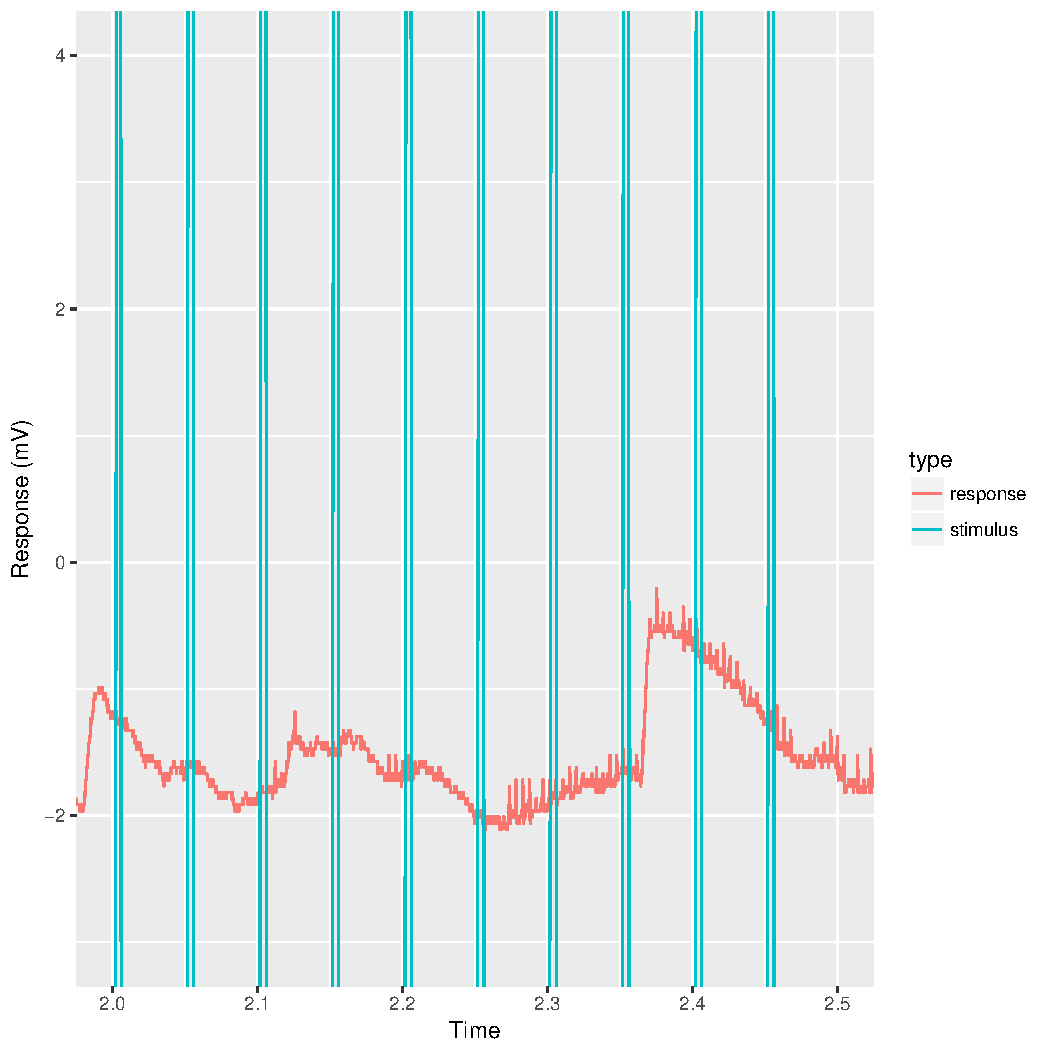
\includegraphics[width = 0.7\textwidth]{./wave-data-typical.pdf}
    \caption{A sweep with more failures}
  \end{figure}
\end{frame}

%%%%%%%%%%%%%%%%%%%%%%%%%%%%%%%%%%%%%%%%%%%%%%%%%%%%%%%%%%%%%%%%%%%%%%%%%%%%%%%%
% Classical Mathematical Models for the Distribution Don't Work
%%%%%%%%%%%%%%%%%%%%%%%%%%%%%%%%%%%%%%%%%%%%%%%%%%%%%%%%%%%%%%%%%%%%%%%%%%%%%%%%

\section{Applying the Compound Binomial Distribution Model}

\subsection{Introducing the Model}

\begin{frame}{Compound Binomial Distribution Model}
  % Explain the binomial distribution model in picture and with equations
  \begin{figure}
    \centering
    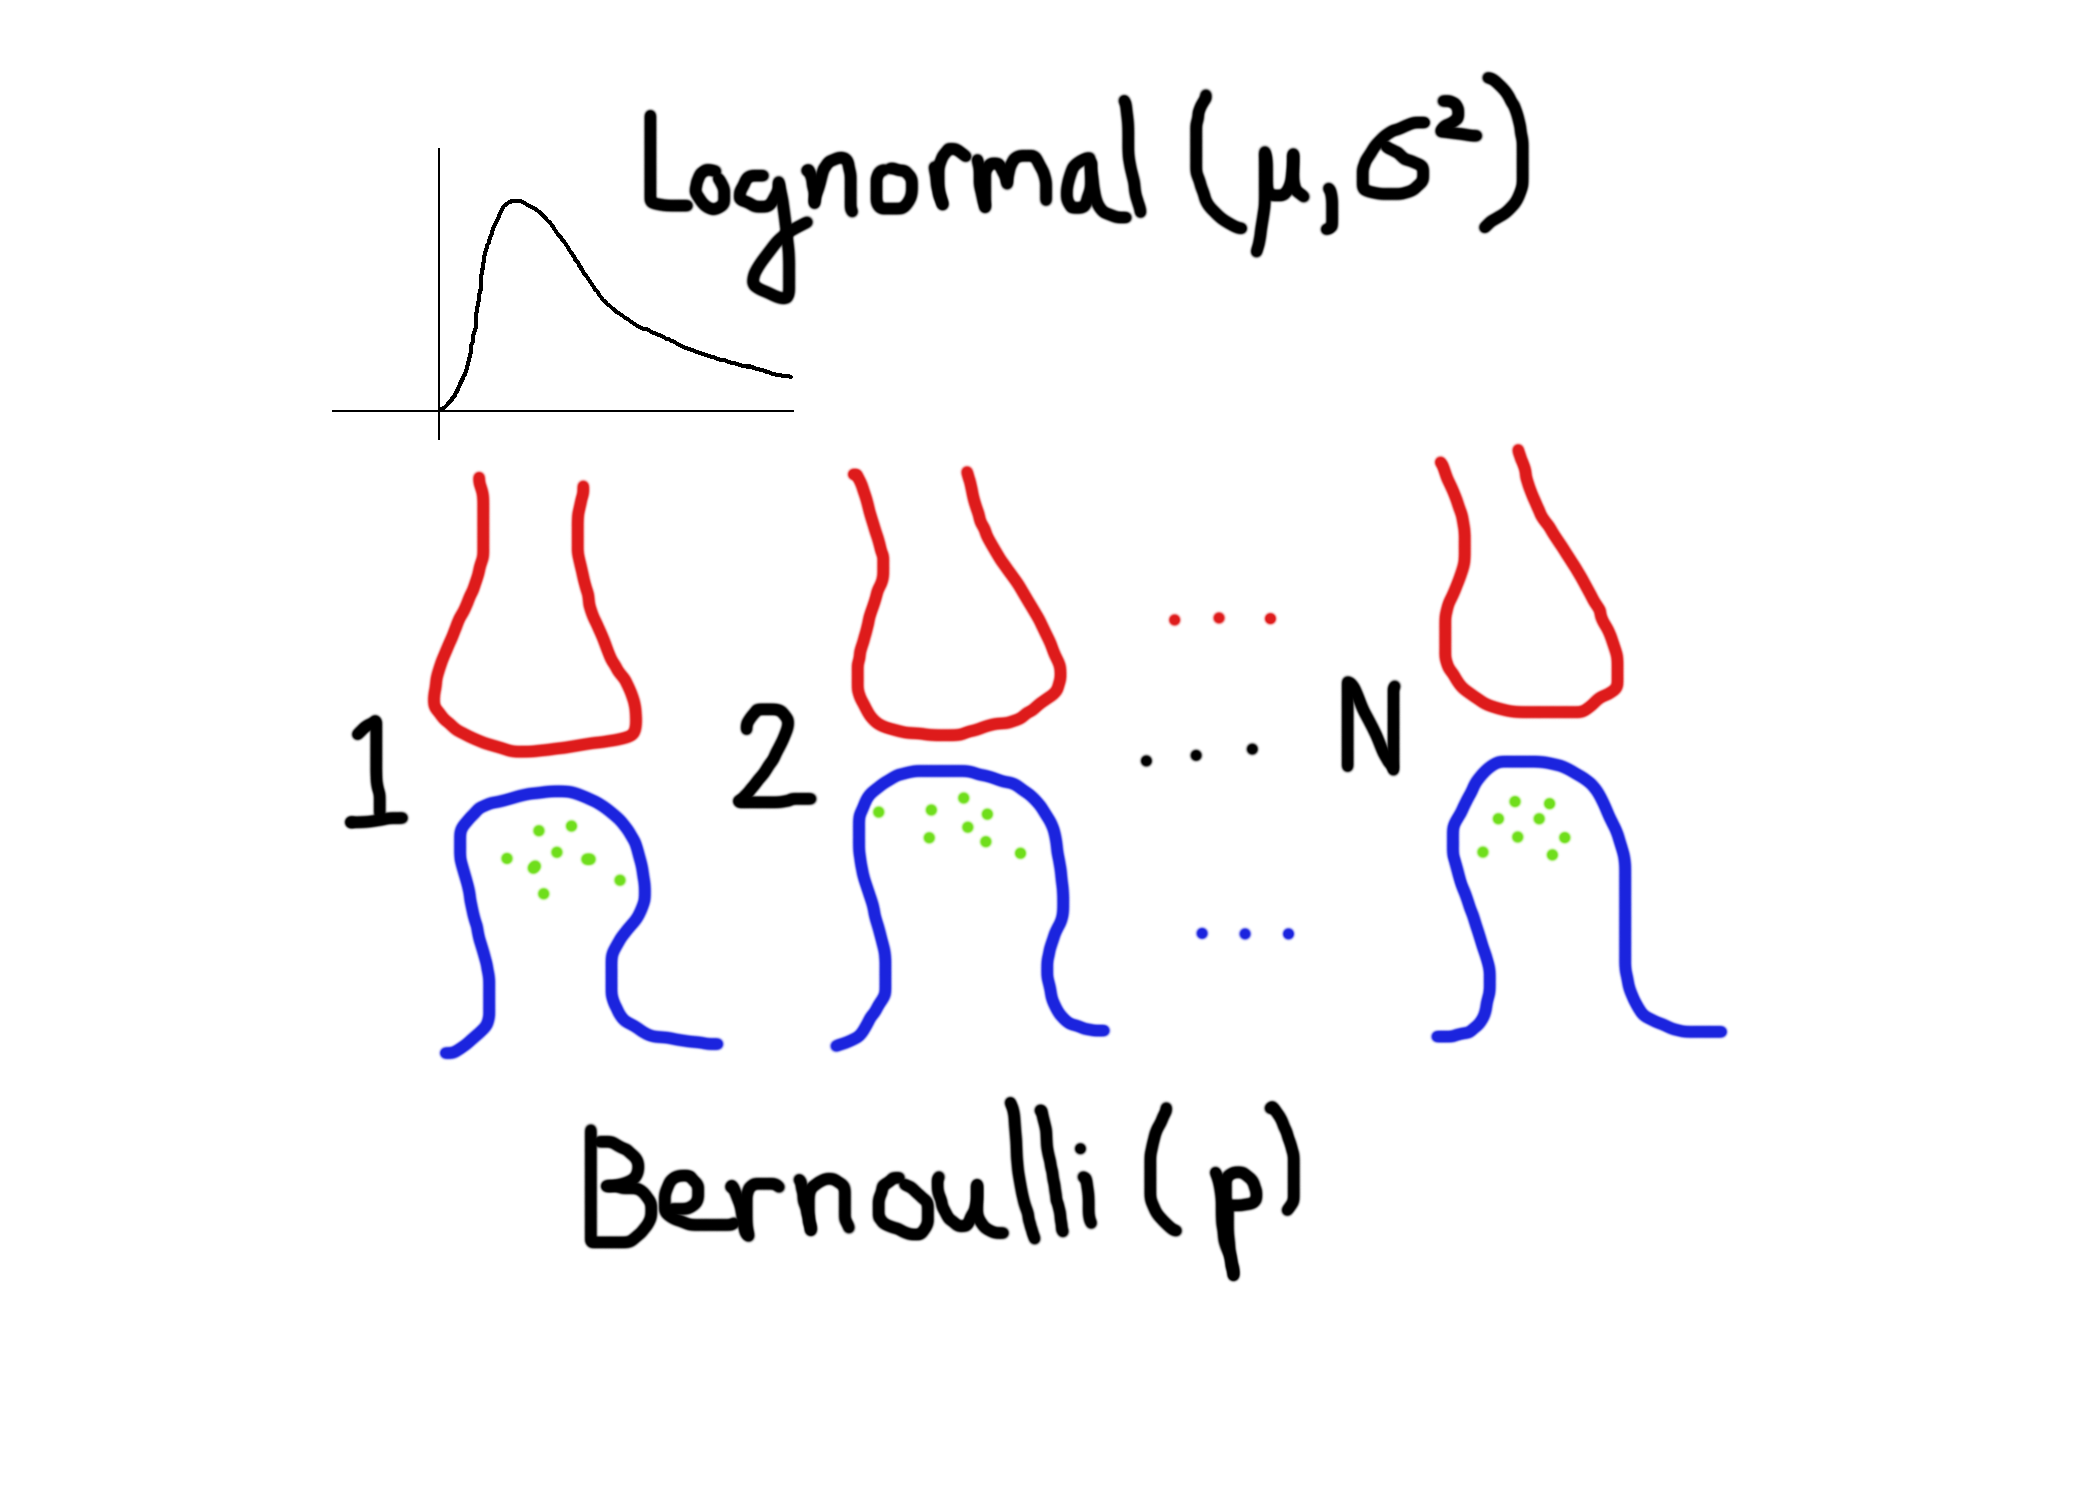
\includegraphics[width = 0.7\textwidth]{./compound-binomial-distribution.png}
    \caption{Compound binomial distribution model}
  \end{figure}
\end{frame}

\begin{frame}{Mathematical Description}
  \[
    X = \sum_{j=1}^N X_j, Y_j\sim\Bernoulli(p), 
    \begin{cases}
      (X_j\mid Y_j = 1)\sim\Lognormal(\mu, \sigma^2) \\ 
      (X_j\mid Y_j = 0)\sim0
    \end{cases}
  \]
\end{frame}

\subsection{Application to our Data}

\begin{frame}{Post-synaptic Amplitude Distribution Over Trials}
  % Histogram showing high failure rate
  \begin{figure}
    \centering
    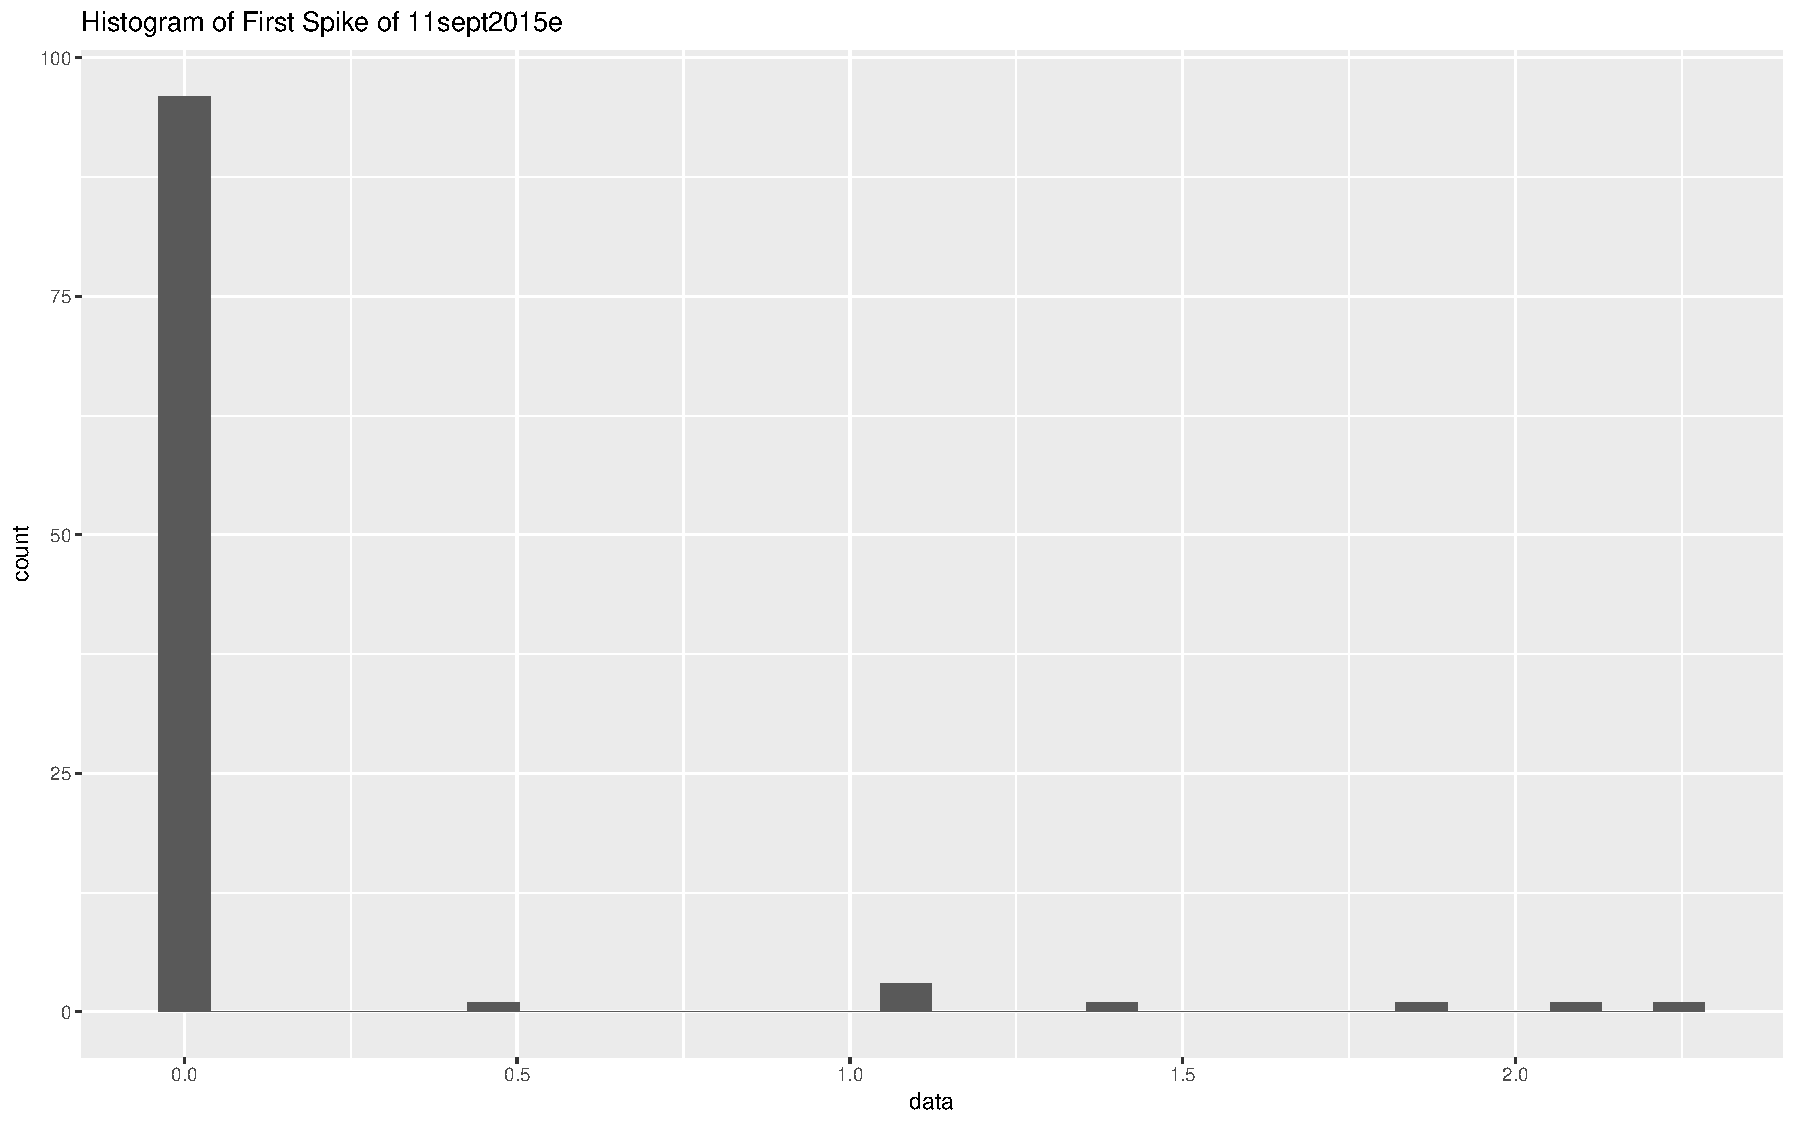
\includegraphics[width = 0.7\textwidth]{./histogram.pdf}
    \caption{Example of observed distribution}
  \end{figure}
\end{frame}

\begin{frame}{Inference of Parameters Assuming the Binomial Model}
  % Explain method of moments extraction of parameters
  \begin{itemize}
    \item Method of Moments guesses the parameters $\mu, \sigma^2, p$ by matching sample properties to the theoretical values of the properties. 
    \item In our case, we match the failure rate, mean value, and variance. 
    \item If $p_f$ is the failure rate, $\overline X$ is the sample mean, and $S^2$ is the sample variance, then
    \[
      p = 1 - \sqrt[N]{p_f}
    \]
    \[
      \begin{pmatrix}\mu\\\sigma\end{pmatrix} = \begin{pmatrix}-1&1\\2&-1\end{pmatrix}\begin{pmatrix}\frac12\log\left(\frac{S^2}{Np} + \left(\frac{\overline X}{Np}\right)^2\right)\\2\log\left(\frac{\overline X}{Np}\right)\end{pmatrix}. 
    \]
  \end{itemize}
\end{frame}

\begin{frame}{Inference of Parameters on Simulated Data}
  % Show that inference of parameters works if it truly comes from this model
  \begin{figure}
    \centering
    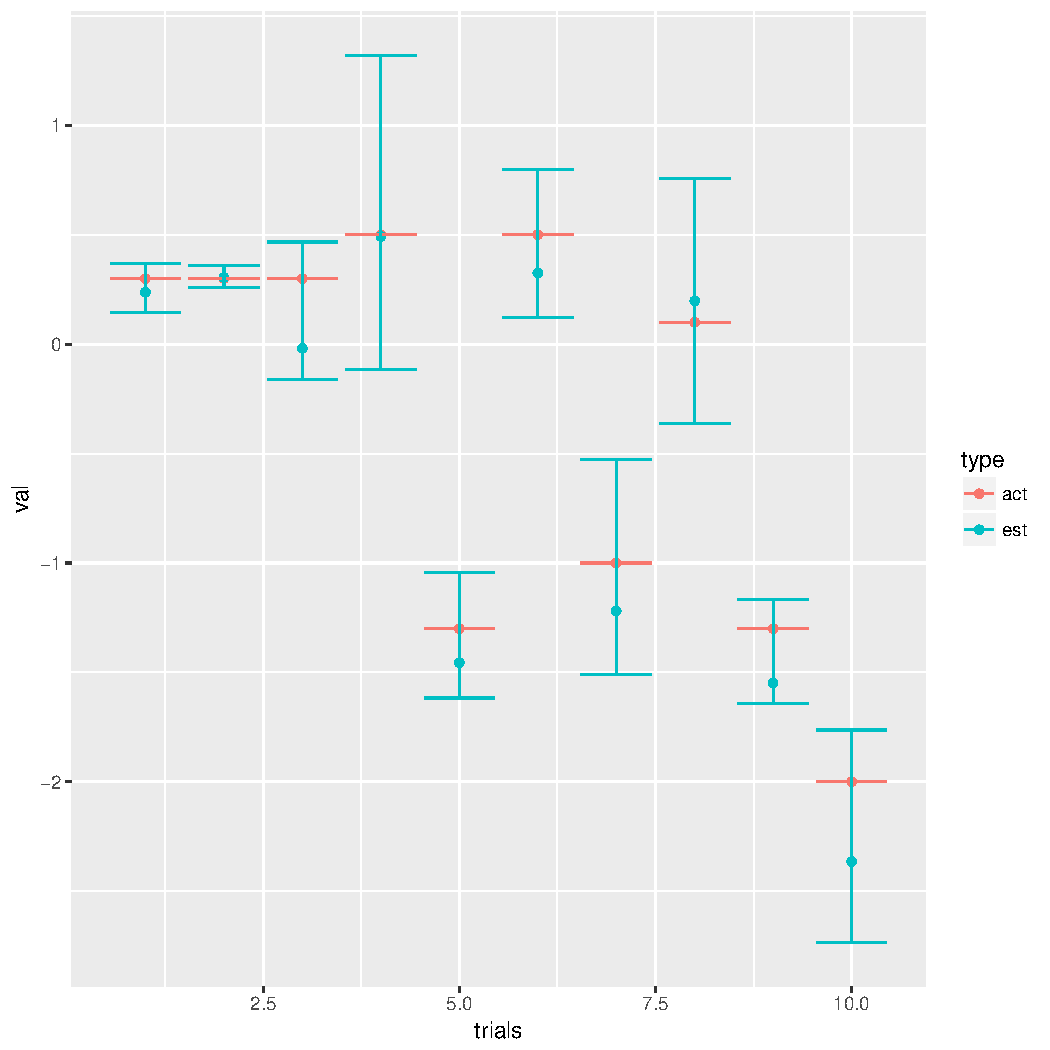
\includegraphics[width = 0.7\textwidth]{./mu-100-samples.pdf}
    \caption{Inferring $\mu$}
  \end{figure}
\end{frame}

\begin{frame}{Inference of Parameters on Simulated Data}
  % Show that inference of parameters works if it truly comes from this model
  \begin{figure}
    \centering
    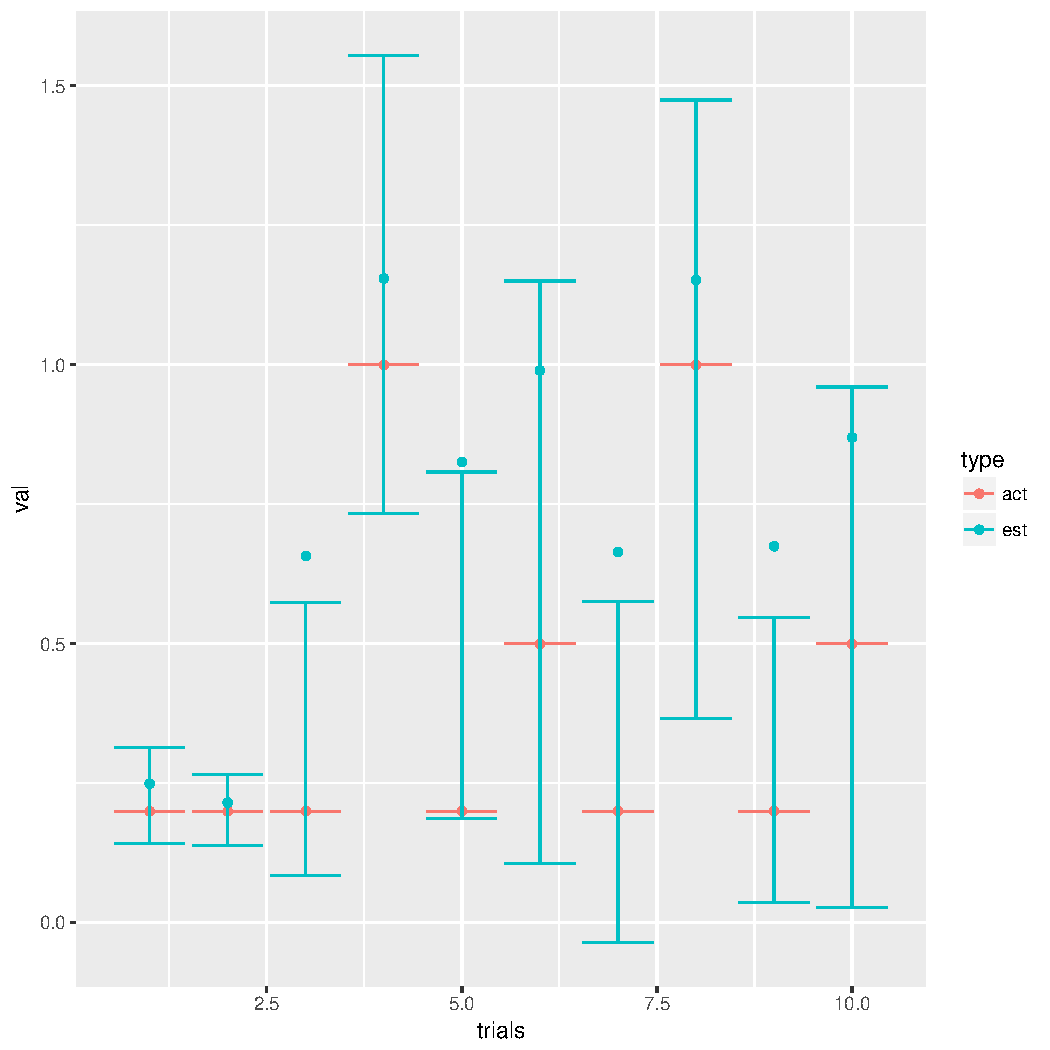
\includegraphics[width = 0.7\textwidth]{./sigma-100-samples.pdf}
    \caption{Inferring $\sigma$}
  \end{figure}
\end{frame}

\begin{frame}{Inference of Parameters on Simulated Data}
  % Show that inference of parameters works if it truly comes from this model
  \begin{figure}
    \centering
    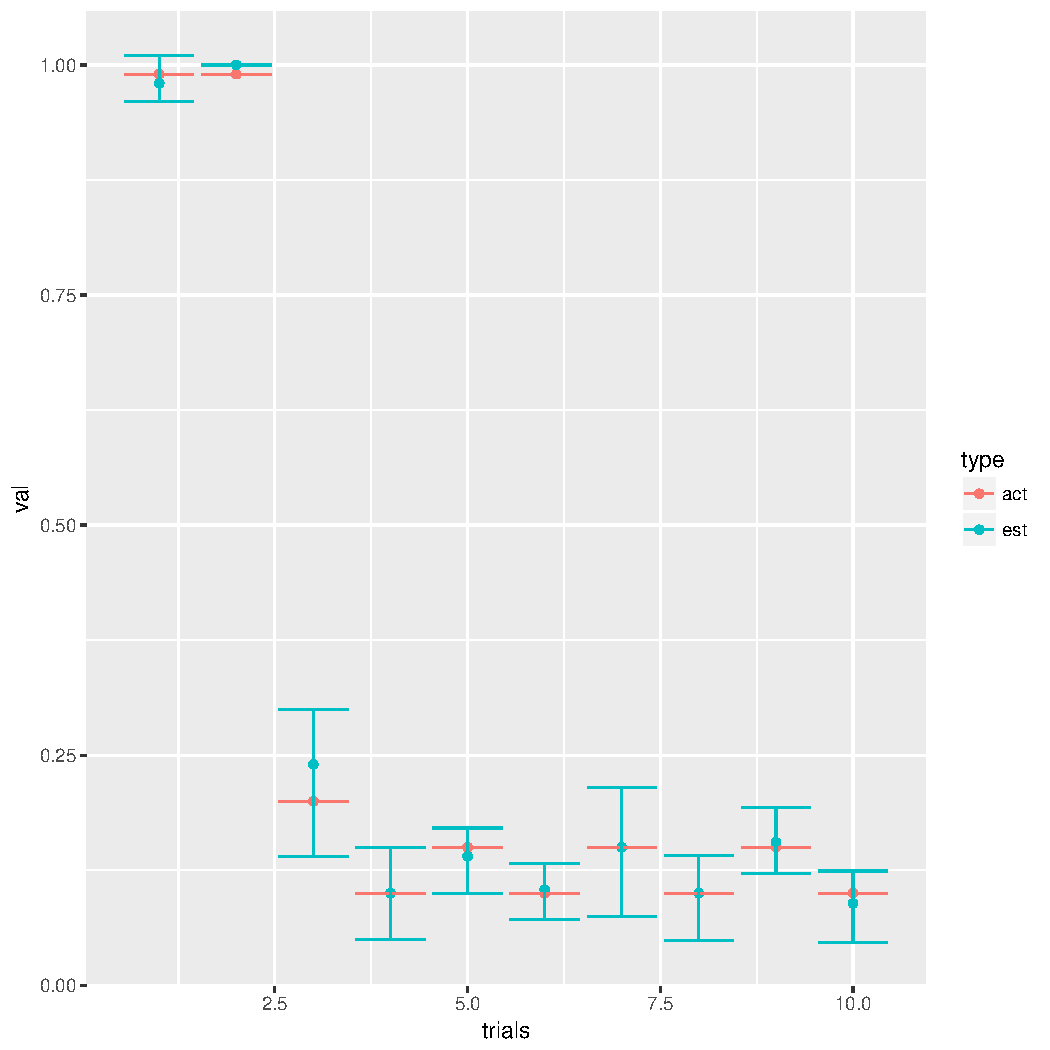
\includegraphics[width = 0.7\textwidth]{./p-100-samples.pdf}
    \caption{Inferring $p$}
  \end{figure}
\end{frame}

\begin{frame}{Comparison of Simulated Model Against the Data}
  % Histogram of simulation vs original data
  \begin{figure}
    \centering
    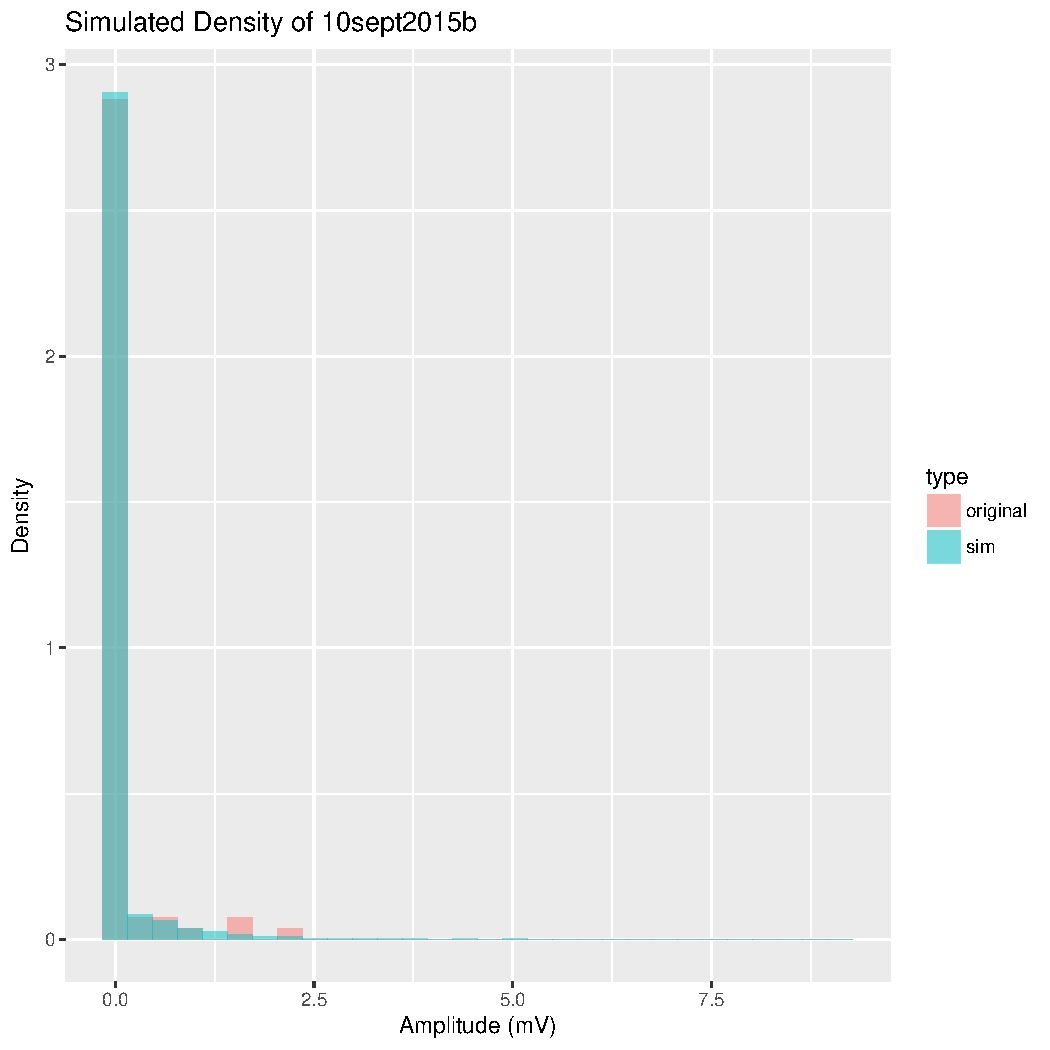
\includegraphics[width = 0.7\textwidth]{./10sept2015b-sim-vs-original-N=2-spike2.pdf}
    \caption{Simulating from the inferred model}
  \end{figure}
\end{frame}

\begin{frame}{Comparison of Simulated Model Against the Data}
  % Probabilities against N
  \begin{figure}
    \centering
    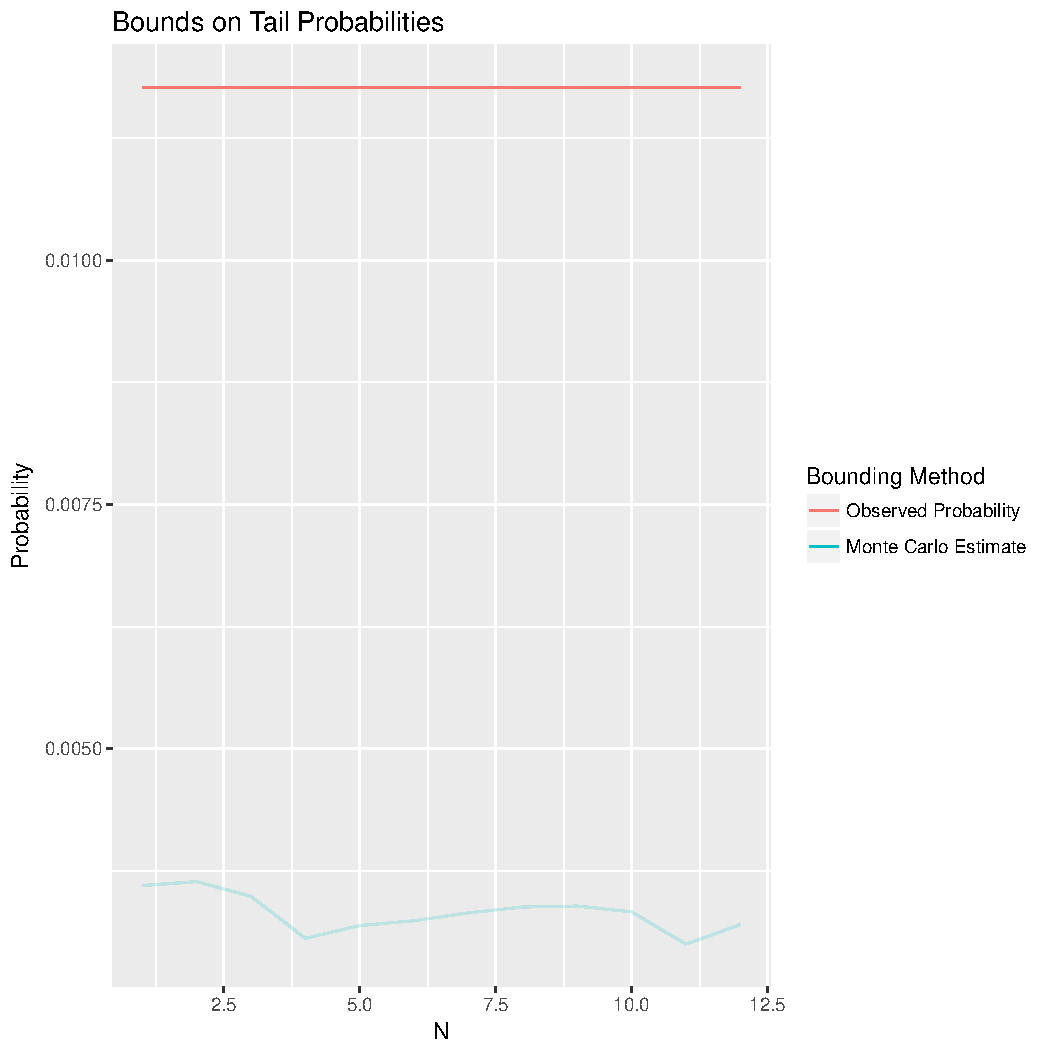
\includegraphics[width = 0.7\textwidth]{./10sept2015b-max-amp-sim-first-col.pdf}
    \caption{Monte Carlo estimate of tail probabilities}
  \end{figure}
\end{frame}


\end{document}
